\documentclass{ximera}

\usepackage[a4paper,left=1.5cm,right=1.5cm]{geometry}
\usepackage{amsmath}
\usepackage{amssymb}
\usepackage{ifthen}
\usepackage{environ}
\usepackage{multicol}
\usepackage{tikz} 
\usepackage{pgfplots} 
\usepackage{enumitem}
\pgfplotsset{compat=1.18}

\renewenvironment{exercise}[1][2in]
{
    \stepcounter{problem@Depth}
    \begin{trivlist}
    \item[\normalfont\bfseries Oefening\hspace{0.2em}\problemNumber)]
    \leavevmode\par
    \normalfont
}
{
    \problemEnvironmentEnd
}

\renewenvironment{solution}
{
    \ifhandout
        \setbox0\vbox\bgroup
    \else
        \begin{trivlist}
        \item[\normalfont\bfseries Oplossing:]
        \leavevmode\par
        \normalfont
    \fi
}
{
    \ifhandout
        \egroup
    \else
        \end{trivlist}
    \fi
}

\renewenvironment{question}
{
    \stepcounter{problem@Depth}
    \begin{trivlist}
    \item[\normalfont\bfseries Vraag\hspace{0.2em}\problemNumber)]
    \leavevmode\par
    \normalfont
}
{
    \problemEnvironmentEnd
}

\usepackage{fancyhdr}

\pagestyle{fancy}
\fancyhf{}

% Left footer
\fancyfoot[L]{%
    \small Monitoraat geneeskunde
}

% Right footer
\fancyfoot[R]{%
    \small
    Bij vragen: \texttt{arne.vandamme@kuleuven.be}
}

% Footer styling
\renewcommand{\headrulewidth}{0pt}
\renewcommand{\footrulewidth}{0.4pt}

% Apply identical footer to plain pages (e.g. first page)
\fancypagestyle{plain}{%
    \fancyhf{}
    \fancyfoot[L]{\small Monitoraat Geneeskunde}
    \fancyfoot[R]{%
        \small
        Bij vragen: \texttt{arne.vandamme@kuleuven.be}
    }
    \renewcommand{\headrulewidth}{0pt}
    \renewcommand{\footrulewidth}{0.4pt}
}

\usepackage{graphicx}


\begin{document}

\definecolor{drawcolour}{RGB}{0,0,255}
\definecolor{Liquiduscolour}{RGB}{0,160,0}
\definecolor{Soliduscolour}{RGB}{255,0,0}

\begin{center}
    {\Large\textbf{Fasediagrammen \& Hefboomregel}}
\end{center}

\medskip



\begin{exercise}

Hoeveel procent Liquidus bevat een legering van Ni en Cu met $70\%$ massa Ni bij $1380$°C? Maak een schatting aan de hand van het gegeven fasediagram van Ni en Cu.


\bigskip
\begin{center}
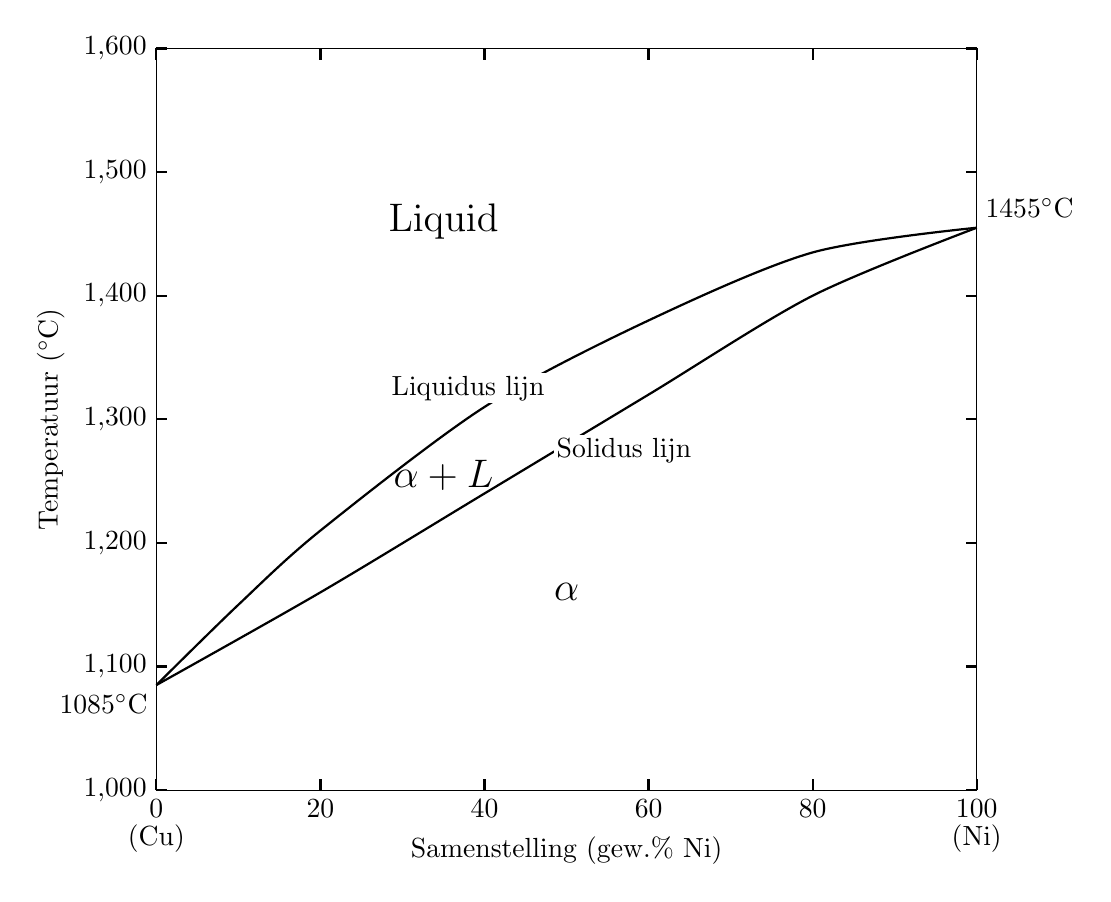
\begin{tikzpicture}
\begin{axis}[
    width=12cm, height=11cm, xmin=0, xmax=100, ymin=1000, ymax=1600,
    xlabel={Samenstelling (gew.\% Ni)}, ylabel={Temperatuur ($^\circ$C)},
    xtick={0,20,40,60,80,100},
    ytick={1000,1100,1200,1300,1400,1500,1600},
    axis lines=box, tick style={black,thick},
    major tick length=4pt, enlargelimits=false, clip=false,
]

% Liquidus
\addplot[thick, smooth] coordinates {
    (0,1085) (10,1150) (20,1210) (40,1310)
    (60,1380) (80,1435) (100,1455)
};

% Solidus
\addplot[thick, smooth] coordinates {
    (0,1085) (20,1160) (40,1240)
    (60,1320) (80,1400) (100,1455)
};

% Region labels
\node at (axis cs:35,1460) {\Large Liquid};
\node at (axis cs:35,1255) {\Large $\alpha + L$};
\node at (axis cs:50,1160) {\Large $\alpha$};

% Curve labels
\node[fill=white,inner sep=1pt] at (axis cs:38,1325) {Liquidus lijn};
\node[fill=white,inner sep=1pt] at (axis cs:57,1275) {Solidus lijn};

% Melting point annotations
\node[anchor=north west] at (axis cs:-13,1085) {1085$^\circ$C};
\node[anchor=south east] at (axis cs:113,1455) {1455$^\circ$C};

% Cu and Ni labels
\node[below] at (axis cs:0,980) {(Cu)};
\node[below] at (axis cs:100,980) {(Ni)};

\end{axis}
\end{tikzpicture}
\end{center}
\bigskip

\begin{solution}

Met de hefboomregel kunnen we bepalen welk percentage van de legering vloeibaar is. We trekken hiervoor een verticale lijn op de gegeven procentuele samenstelling.

Het mengsel van Cu en Ni koelt af vanuit de Liquidus fase naar de solidus fase ($\alpha$ fase).

\begin{center}
\begin{tikzpicture}
\begin{axis}[
    width=12cm, height=11cm, xmin=0, xmax=100, ymin=1000, ymax=1600,
    xlabel={Samenstelling (gew.\% Ni)}, ylabel={Temperatuur ($^\circ$C)},
    xtick={0,20,40,60,80,100},
    ytick={1000,1100,1200,1300,1400,1500,1600},
    axis lines=box, tick style={black,thick},
    major tick length=4pt, enlargelimits=false, clip=false,
]

% Liquidus
\addplot[thick, smooth] coordinates {
    (0,1085) (10,1150) (20,1210) (40,1310)
    (60,1380) (80,1435) (100,1455)
};

% Solidus
\addplot[thick, smooth] coordinates {
    (0,1085) (20,1160) (40,1240)
    (60,1320) (80,1400) (100,1455)
};

% C0 lines
\addplot[drawcolour, thin, no marks]
    coordinates {(0,1380) (100,1380)};
\addplot[drawcolour, thin, no marks]
    coordinates {(70,1000) (70,1600)};

% Region labels
\node at (axis cs:35,1460) {\Large Liquid};
\node at (axis cs:35,1255) {\Large $\alpha + L$};
\node at (axis cs:50,1160) {\Large $\alpha$};

\node[drawcolour,font=\bfseries,yshift=-8pt]
    at (axis cs:70,1000) {70};
% Points
\addplot[only marks, mark=*, drawcolour, mark size=2pt]
    coordinates {(70,1410)};
\addplot[only marks, mark=*, drawcolour, mark size=2pt]
    coordinates {(70,1380)};
\addplot[only marks, mark=*, drawcolour, mark size=2pt]
    coordinates {(70,1360)};

\node[above left, drawcolour] at (axis cs:70,1410) {A};
\node[above right, drawcolour] at (axis cs:70,1380) {P};
\node[below left, drawcolour] at (axis cs:70,1360) {B};

\end{axis}
\end{tikzpicture}
\end{center}
\bigskip


Tot en met punt A is de stof volledig vloeibaar en vanaf punt B is de stof volledig vast. We kunnnen dus een L en $\alpha$ lijn tekenen om te laten zien dat de stof $100\%$ vloeibaar of vast is.

\begin{center}
\begin{tikzpicture}
\begin{axis}[
    width=12cm, height=11cm, xmin=0, xmax=100, ymin=1000, ymax=1600,
    xlabel={Samenstelling (gew.\% Ni)}, ylabel={Temperatuur ($^\circ$C)},
    xtick={0,20,40,60,80,100},
    ytick={1000,1100,1200,1300,1400,1500,1600},
    axis lines=box, tick style={black,thick},
    major tick length=4pt, enlargelimits=false, clip=false,
]

% Liquidus
\addplot[thick, smooth] coordinates {
    (0,1085) (10,1150) (20,1210) (40,1310)
    (60,1380) (80,1435) (100,1455)
};

% Solidus
\addplot[thick, smooth] coordinates {
    (0,1085) (20,1160) (40,1240)
    (60,1320) (80,1400) (100,1455)
};

% C0 lines
\addplot[drawcolour, thin, no marks]
    coordinates {(70,1000) (70,1600)};

% Region labels
\node at (axis cs:35,1460) {\Large Liquid};
\node at (axis cs:35,1255) {\Large $\alpha + L$};
\node at (axis cs:50,1160) {\Large $\alpha$};

\node[drawcolour,font=\bfseries,yshift=-8pt]
    at (axis cs:70,1000) {70};
% Points
\addplot[only marks, mark=*, drawcolour, mark size=2pt]
    coordinates {(70,1410)};
\addplot[only marks, mark=*, drawcolour, mark size=2pt]
    coordinates {(70,1360)};

\node[above left, drawcolour] at (axis cs:70,1410) {A};
\node[below right, drawcolour] at (axis cs:70,1360) {B};

% L and alpha lines
\addplot[Liquiduscolour, ultra thick, no marks]
    coordinates {(70,1410) (83,1410)};
\addplot[Soliduscolour, ultra thick, no marks]
    coordinates {(54,1360) (70,1360)};
\node[Liquiduscolour,font=\bfseries\Large,yshift=10pt]
    at (axis cs:72.5,1410) {L};
\node[Soliduscolour,font=\bfseries\Large,yshift=10pt]
    at (axis cs:65,1360) {$\alpha$};
\addplot[only marks, mark=*, Liquiduscolour, mark size=2pt]
    coordinates {(83,1410)};
\addplot[only marks, mark=*, Soliduscolour, mark size=2pt]
    coordinates {(54,1360)};

\end{axis}
\end{tikzpicture}
\end{center}
\bigskip


Op het gevraagde punt is de stof deels vast en deels vloeibaar. We tekenen daarom een \textcolor{Liquiduscolour}{\textbf{L}} lijn en een \textcolor{Soliduscolour}{\textbf{$\alpha$}} lijn. Let op: een veel gemaakte fout is het omwisselen van deze twee lijnen.


\bigskip
\begin{center}
\begin{tikzpicture}
\begin{axis}[
    width=12cm, height=11cm, xmin=0, xmax=100, ymin=1000, ymax=1600,
    xlabel={ (gew.\% Ni) \quad}, ylabel={Temperatuur ($^\circ$C)},
    xtick={0,20,40,80,100},
    ytick={1000,1100,1200,1300,1400,1500,1600},
    axis lines=box, tick style={black,thick},
    major tick length=4pt, enlargelimits=false, clip=false,
]

% Liquidus
\addplot[thick, smooth] coordinates {
    (0,1085) (10,1150) (20,1210) (40,1310)
    (60,1380) (80,1435) (100,1455)
};

% Solidus
\addplot[thick, smooth] coordinates {
    (0,1085) (20,1160) (40,1240)
    (60,1320) (80,1400) (100,1455)
};

% C0 lines
\addplot[drawcolour, thin, no marks]
    coordinates {(0,1380) (100,1380)};
\addplot[drawcolour, thin, no marks]
    coordinates {(70,1000) (70,1600)};

% CL line
\addplot[Soliduscolour, thin, no marks]
    coordinates {(60,1000) (60,1600)};

% Calpha line
\addplot[Liquiduscolour, thin, no marks]
    coordinates {(75,1000) (75,1600)};

% L and alpha lines
\addplot[Liquiduscolour, ultra thick, no marks]
    coordinates {(70,1380) (75,1380)};
\addplot[Soliduscolour, ultra thick, no marks]
    coordinates {(60,1380) (70,1380)};

% Total line
\addplot[drawcolour, ultra thick, no marks]
    coordinates {(60,1115) (75,1115)};

% Region labels
\node at (axis cs:35,1460) {\Large Liquid};
\node at (axis cs:35,1255) {\Large $\alpha + L$};
\node at (axis cs:50,1160) {\Large $\alpha$};

% Composition labels
\node[Soliduscolour,font=\bfseries,yshift=-8pt]
    at (axis cs:60,1000) {60};
\node[Soliduscolour,font=\bfseries,yshift=-8pt]
    at (axis cs:60,970) {$C_L$};

\node[drawcolour,font=\bfseries,yshift=-8pt]
    at (axis cs:70,1000) {70};
\node[drawcolour,font=\bfseries,yshift=-8pt]
    at (axis cs:70,970) {$C_0$};

\node[Liquiduscolour,font=\bfseries,yshift=-8pt]
    at (axis cs:75,1000) {75};
\node[Liquiduscolour,font=\bfseries,yshift=-8pt]
    at (axis cs:75,970) {$C_{\alpha}$};

% Phase labels
\node[Liquiduscolour,font=\bfseries\Large,yshift=10pt]
    at (axis cs:72.5,1380) {L};
\node[Soliduscolour,font=\bfseries\Large,yshift=10pt]
    at (axis cs:65,1380) {$\alpha$};

\node[drawcolour,font=\bfseries\Large,yshift=-12pt]
    at (axis cs:67.5,1115) {tot};

% Points
\addplot[only marks, mark=*, drawcolour, mark size=2pt]
    coordinates {(70,1380)};
\addplot[only marks, mark=*, Liquiduscolour, mark size=2pt]
    coordinates {(75,1380)};
\addplot[only marks, mark=*, Soliduscolour, mark size=2pt]
    coordinates {(60,1380)};

\end{axis}
\end{tikzpicture}
\end{center}
\bigskip

We definiëren hier de volgende punten op de horizontale as:

\begin{itemize}
    \item $C_0 = 70$ = oorspronkelijke samenstelling ($70$ gew.\% Ni)
    \item $C_L = 60$ = samenstelling van de vloeibare fase
    \item $C_{\alpha} = 75$ = samenstelling van de vaste fase
\end{itemize}

Met deze punten kunnen we de volgende afstanden definiëren op het diagram:

\begin{itemize}
    \item $\textcolor{drawcolour}{\mathbf{\text{\textbf{tot}}}} = 75 - 60$ = totale hoeveelheid stof
    \item $\textcolor{Liquiduscolour}{\mathbf{\text{\textbf{L}}}} = 75 - 70$ = hoeveelheid vloeibare fase
    \item $\textcolor{Soliduscolour}{\boldsymbol{\alpha}} = 70 - 60$ = hoeveelheid vaste fase
\end{itemize}

Nu zoeken we het percentage vloeibare fase. Hiervoor gebruiken we de lengte van het vloeibare gedeelte ($\textcolor{Liquiduscolour}{\mathbf{\text{\textbf{L}}}}$) ten opzichte van de totale lengte ($\textcolor{drawcolour}{\mathbf{\text{\textbf{tot}}}}$).

\[
\text{hoeveelheid vloeibare fase}
=
\frac{\textcolor{Liquiduscolour}{\mathbf{\text{\textbf{L}}}}}
{\textcolor{drawcolour}{\mathbf{\text{\textbf{tot}}}}}
=
\frac{C_{\alpha}-C_0}{C_{\alpha}-C_L}
=
\frac{75-70}{75-60}
=
\frac{5}{15}
=
0{,}333
\]

Deze legering bevat bij $1380$°C dus ongeveer $33\%$ vloeibare fase (Liquidus) en $66\%$ vaste $\alpha$-fase.

\end{solution}

\end{exercise}



\begin{exercise}

Een mengeling met $20\%$ massa Si en $80\%$ massa Ge wordt afgekoeld van $1500$°C. Tot hoeveel graden moet er gekoeld worden zodat ongeveer $66\%$ van de vloeistof gestold is? Maak een schatting aan de hand van het gegeven fasediagra van Si en Ge. Teken de microstructuur van deze samenstelling.

\bigskip
\begin{center}
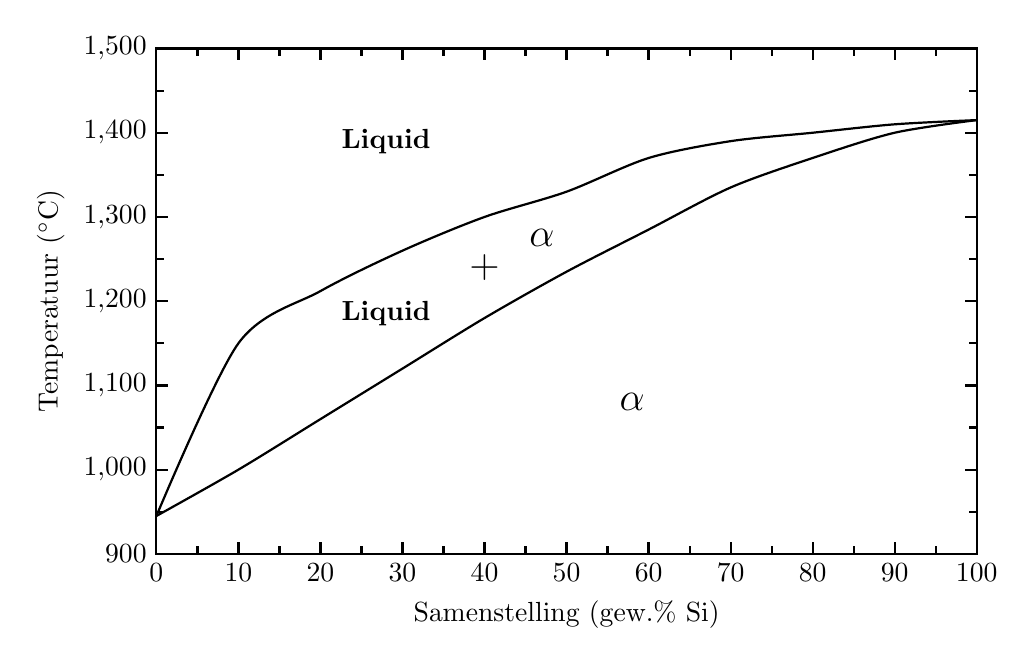
\begin{tikzpicture}
\begin{axis}[
    width=12cm, height=8cm, xmin=0, xmax=100, ymin=900, ymax=1500,
    xlabel={Samenstelling (gew.\% Si)}, ylabel={Temperatuur ($^\circ$C)},
    xtick={0,10,20,30,40,50,60,70,80,90,100},
    ytick={900,1000,1100,1200,1300,1400,1500},
    minor tick num=1, tick style={black,thick}, axis line style={black,thick},
    enlargelimits=false, clip=false,
]

% Liquidus
\addplot[smooth, thick, black] coordinates {
    (0,945) (10,1150) (20,1212) (30,1260) (40,1300) (50,1330)
    (60,1370) (70,1390) (80,1400) (90,1410) (100,1415)
};

% Solidus
\addplot[smooth, thick, black] coordinates {
    (0,945) (10,1000) (20,1060) (30,1120) (40,1180) (50,1235)
    (60,1285) (70,1335) (80,1370) (90,1400) (100,1415)
};

% Phase labels
\node at (axis cs:28,1390) {\bfseries Liquid};
\node at (axis cs:40,1240) {\Large $+$};
\node at (axis cs:28,1185) {\bfseries Liquid};
\node at (axis cs:47,1275) {\Large $\alpha$};
\node at (axis cs:58,1080) {\Large $\alpha$};

\end{axis}
\end{tikzpicture}
\end{center}
\bigskip


\begin{solution} %%%%%%%%%%%%%%%%%%%%%%%%%%%%%%%%%%%%%%%%%%%%%%%%%%%%%%%%%%%%%%%%%%%%%%%%%%%%%%%%%%%%%%%%%%

\begin{center}
\begin{tikzpicture}
\begin{axis}[
    width=12cm, height=8cm, xmin=0, xmax=100, ymin=900, ymax=1500,
    xlabel={Samenstelling (gew.\% Si)}, ylabel={Temperatuur ($^\circ$C)},
    xtick={0,10,20,30,40,50,60,70,80,90,100},
    ytick={900,1000,1100,1200,1300,1400,1500},
    minor tick num=1, tick style={black,thick}, axis line style={black,thick},
    enlargelimits=false, clip=false,
]

% Liquidus
\addplot[smooth, thick, black] coordinates {
    (0,945) (10,1150) (20,1212) (30,1260) (40,1300) (50,1330)
    (60,1370) (70,1390) (80,1400) (90,1410) (100,1415)
};

% Solidus
\addplot[smooth, thick, black] coordinates {
    (0,945) (10,1000) (20,1060) (30,1120) (40,1180) (50,1235)
    (60,1285) (70,1335) (80,1370) (90,1400) (100,1415)
};

% C0 lines
\addplot[drawcolour, thin, no marks] coordinates {(0,1100) (100,1100)};
\addplot[drawcolour, thin, no marks] coordinates {(20,900) (20,1500)};

% CL line
\addplot[Soliduscolour, thin, no marks] coordinates {(8,900) (8,1500)};

% Calpha line
\addplot[Liquiduscolour, thin, no marks] coordinates {(26,900) (26,1500)};

% L line
\addplot[Soliduscolour, ultra thick, no marks] coordinates {(8,1350) (20,1350)};

% alpha line
\addplot[Liquiduscolour, ultra thick, no marks] coordinates {(20,1350) (26,1350)};

% tot line
\addplot[drawcolour, ultra thick, no marks] coordinates {(8,950) (26,950)};

% Phase labels
\node at (axis cs:28,1390) {\bfseries Liquid};
\node at (axis cs:40,1240) {\Large $+$};
\node at (axis cs:28,1185) {\bfseries Liquid};
\node at (axis cs:47,1275) {\Large $\alpha$};
\node at (axis cs:58,1080) {\Large $\alpha$};

% Composition labels
\node[Soliduscolour,font=\bfseries,yshift=-8pt] at (axis cs:8,900) {8};
\node[Soliduscolour,font=\bfseries,yshift=-8pt] at (axis cs:8,860) {$C_L$};
\node[Liquiduscolour,font=\bfseries,yshift=-8pt] at (axis cs:26,900) {26};
\node[Liquiduscolour,font=\bfseries,yshift=-8pt] at (axis cs:26,860) {$C_{\alpha}$};
\node[drawcolour,font=\bfseries,yshift=-8pt] at (axis cs:20,860) {$C_0$};

\node[Soliduscolour,font=\bfseries\Large,yshift=-8pt] at (axis cs:14,1350) {$\alpha$};
\node[Liquiduscolour,font=\bfseries\Large,yshift=-8pt] at (axis cs:23,1350) {L};
\node[drawcolour,font=\bfseries\Large,yshift=-8pt] at (axis cs:17,950) {tot};

\addplot[only marks, mark=*, drawcolour, mark size=2pt] coordinates {(20,1100)};
\addplot[only marks, mark=*, Soliduscolour, mark size=2pt] coordinates {(8,1100)};
\addplot[only marks, mark=*, Liquiduscolour, mark size=2pt] coordinates {(26,1100)};

\end{axis}
\end{tikzpicture}
\end{center}

\bigskip


Met de hefboomregel kunnen we bepalen welk percentage van de legering gestold is. We trekken hiervoor een verticale lijn op de gegeven procentuele samenstelling.

We definiëren hier de volgende punten op de horizontale as (de naamgeving van deze punten is lichtjes verwarrend, dus gebruik gerust je eigen naamgeving):

\begin{itemize}
    \item $C_0 = 20$ = oorspronkelijke samenstelling ($20$ gew.$\%$ Si)
    \item $C_L = 8$ = samenstelling van de vloeibare fase
    \item $C_{\alpha} = 26$ = samenstelling van de vaste fase
\end{itemize}

Met deze punten kunnen we de volgende afstanden deffiniëren op het diagram:

\begin{itemize}
    \item $\textcolor{drawcolour}{\mathbf{\text{\textbf{tot}}}} = 26 - 8$ = totale hoeveelheid stof
    \item $\textcolor{Liquiduscolour}{\mathbf{\text{\textbf{L}}}} = 20 - 8$ = hoeveelheid liquidus fase
    \item $\textcolor{Soliduscolour}{\boldsymbol{\alpha}} = 26 - 20$ = hoeveelheid vaste fase
\end{itemize}

Nu zoeken we de temperatuur waarvoor $66\%$ van de vloeistof gestold is. We trekken een horizontale lijn op de plaats waar $66\%$ van de lijn aan de linkerkant ligt ($\textcolor{Soliduscolour}{\boldsymbol{\alpha}}$). Dit is onze hoeveelheid $\alpha$-fase, dus vaste fase.

\[
\text{hoeveelheid } \alpha\text{-fase} = \frac{\textcolor{Soliduscolour}{\boldsymbol{\alpha}}}{\textcolor{drawcolour}{\mathbf{\text{\textbf{tot}}}}} = \frac{C_L-C_0}{C_L-C_{\alpha}}=0{,}66
\]

Deze samenstelling komt dus voor bij een temperatuur van ongeveer $1100$°C.

De samenstelling bestaat dan uit $66\%$ $\alpha$-fase (grijze korrels op de figuur) en $33\%$ Liquidus-fase (witte vloeistof op de figuur).

\begin{center}
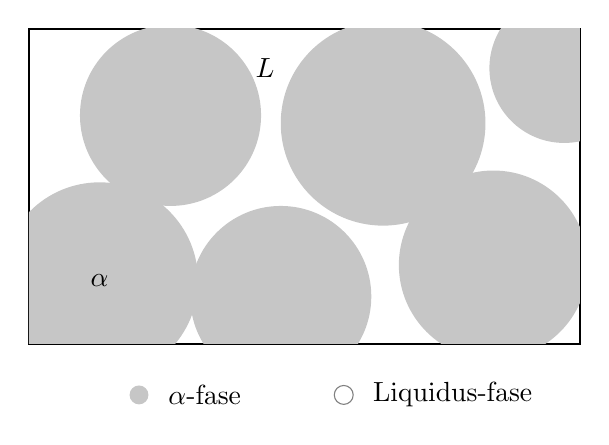
\begin{tikzpicture}
    \draw[thick] (0,0) rectangle (7,4);
    \begin{scope}
        \clip (0,0) rectangle (7,4);
        \foreach \x/\y/\r in {0.9/0.8/1.25, 3.2/0.6/1.15, 5.9/1.0/1.20, 1.8/2.9/1.15, 4.5/2.8/1.30, 6.8/3.5/0.95}{
            \fill[gray!45] (\x,\y) circle (\r);
        }
    \end{scope}
    \node at (0.9,0.8) {$\alpha$};
    \node at (3,3.5) {$L$};
    \fill[gray!45] (1.4,-0.65) circle (0.12);
    \node[anchor=west] at (1.65,-0.65) {$\alpha$-fase};
    \fill[white] (4.0,-0.65) circle (0.12);
    \draw[gray] (4.0,-0.65) circle (0.12);
    \node[anchor=west] at (4.25,-0.65) {Liquidus-fase};
\end{tikzpicture}
\end{center}


\end{solution}

\end{exercise}











\begin{exercise}
    
Gegeven is het fasediagram van Ag en Sn. Beantwoord de onderstaande vragen.


\bigskip
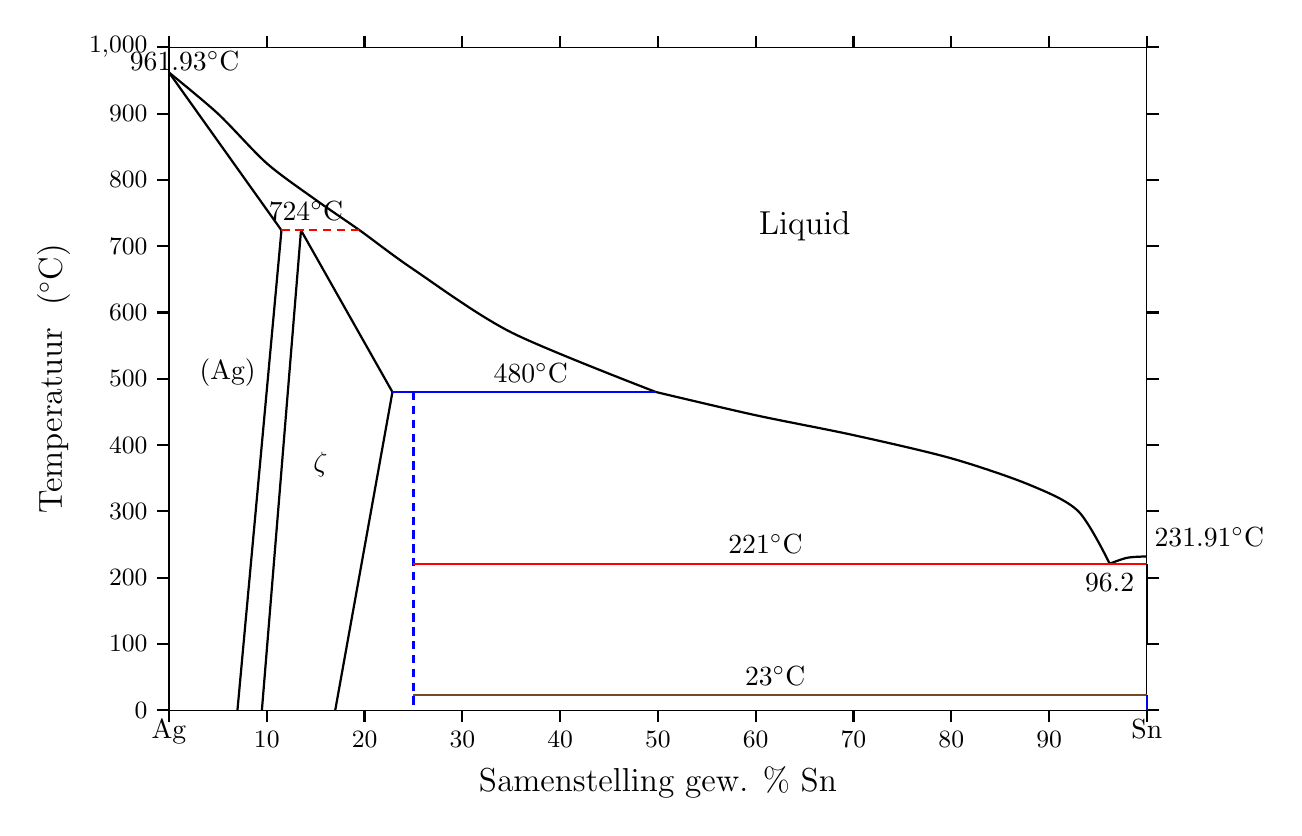
\begin{tikzpicture}
\begin{axis}[
    width=14cm, height=10cm, xmin=0, xmax=100, ymin=0, ymax=1000,
    axis lines=box,
    xlabel={Samenstelling gew. \% Sn}, ylabel={Temperatuur $\ (^\circ\mathrm{C})$},
    xtick={0,10,20,30,40,50,60,70,80,90,100},
    xticklabels={,10,20,30,40,50,60,70,80,90,},
    ytick={0,100,200,300,400,500,600,700,800,900,1000},
    minor tick num=0, tick style={black,thick}, tick align=outside,
    enlargelimits=false, clip=false,
    xlabel style={font=\large}, ylabel style={font=\large},
    tick label style={font=\small},
    every axis plot/.append style={thick, black, no marks},
]

% Liquidus curve
\addplot[smooth] coordinates {(0,962) (5,900) (10,825) (15,770) (19.5,724) (25,665) (35,570) (49.8,480)};
\addplot[smooth] coordinates {(49.8,480) (60,445) (70,415) (80,380) (88,340) (93,300) (96.2,221)};
\addplot[smooth] coordinates {(96.2,221) (98,230) (100,232)};

% Ag-rich phase boundaries
\addplot[smooth] coordinates {(0,962) (11.5,724)};
\addplot[smooth] coordinates {(11.5,724) (7,0)};
\addplot[smooth] coordinates {(13.5,724) (9.5,0)};
\addplot[smooth] coordinates {(13.5,724) (22.85,480)};
\addplot[smooth] coordinates {(22.85,480) (17,0)};
\addplot coordinates {(25,480) (25,0)};

% Horizontal phase boundaries
\addplot coordinates {(11.5,724) (19.5,724)};
\addplot coordinates {(22.85,480) (49.8,480)};
\addplot coordinates {(25,221) (100,221)};
\addplot coordinates {(25,23) (100,23)};

% Sn-rich phase boundaries
\addplot coordinates {(100,221) (100,100)};
\addplot coordinates {(100,23) (100,0)};

% Phase labels
\node at (axis cs:65,730) {\large Liquid};
\node at (axis cs:6,510) {(Ag)};
\node at (axis cs:15.5,370) {$\zeta$};

\node[below] at (axis cs:96.2,221) {96.2};

% Temperature labels
\node[above right] at (axis cs:-5,950) {961.93$^\circ$C};
\node[above] at (axis cs:14,724) {724$^\circ$C};
\node[above] at (axis cs:37,480) {480$^\circ$C};
\node[above] at (axis cs:61,221) {221$^\circ$C};
\node[above left] at (axis cs:113,232) {231.91$^\circ$C};
\node[above] at (axis cs:62,23) {23$^\circ$C};

% Element labels
\node[below] at (axis cs:0,0) {Ag};
\node[below] at (axis cs:100,0) {Sn};

\end{axis}
\end{tikzpicture}
\bigskip

\begin{question}
    Wat is de smelttemperatuur van puur zilver?

    \begin{solution}
        Hiervoor kijken we naar de linkerkant van het diagram, waar staat dat zilver smelt bij $961.93^\circ$C.
    \end{solution}
\end{question}

\begin{question}
    Vanaf welke temperatuur begint een legering met $20\%$ tin te stollen?

    \begin{solution}
        Hiervoor trekken we een verticale lijn op $20\%$ tin en kijken we waar deze de Liquidus lijn snijdt. Dit is op ongeveer $724^\circ$C.

    \bigskip
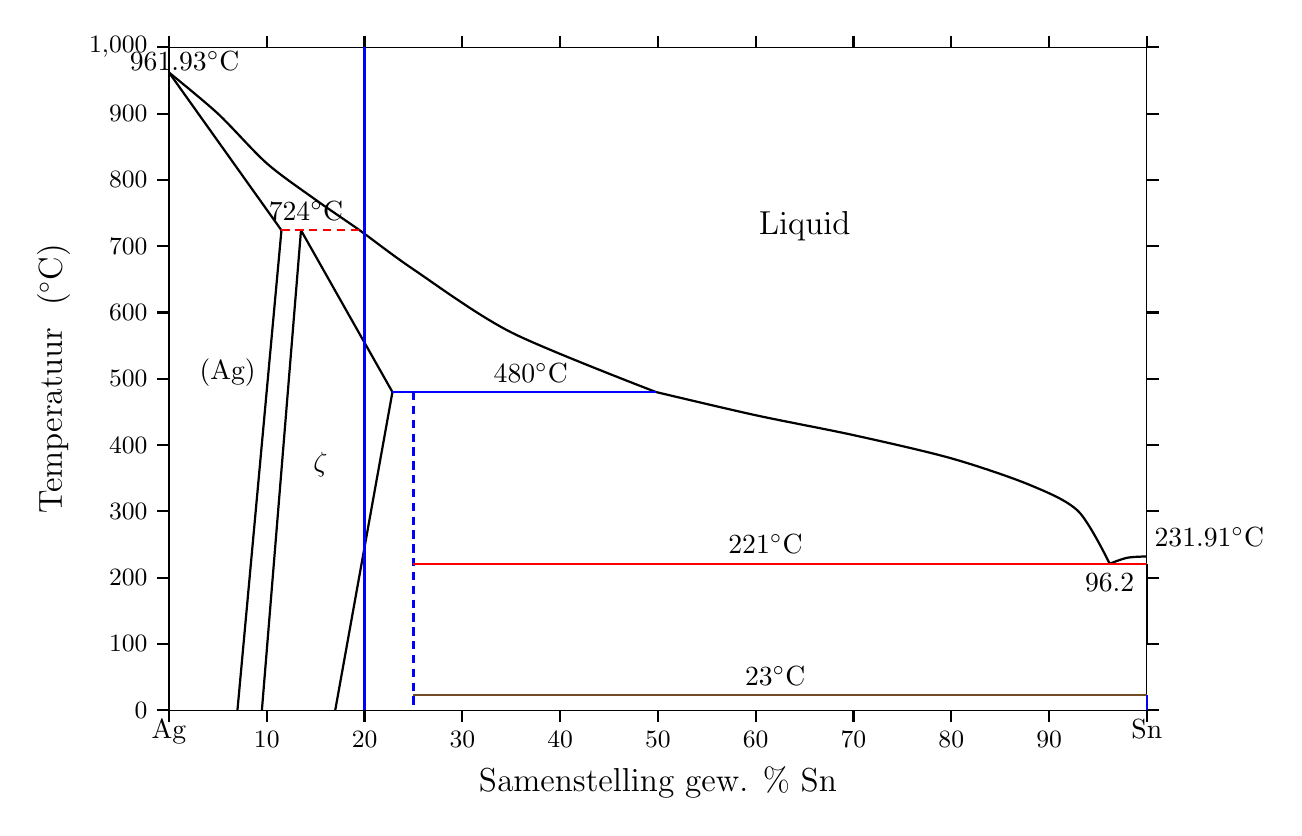
\begin{tikzpicture}
\begin{axis}[
    width=14cm, height=10cm, xmin=0, xmax=100, ymin=0, ymax=1000,
    axis lines=box,
    xlabel={Samenstelling gew. \% Sn}, ylabel={Temperatuur $\ (^\circ\mathrm{C})$},
    xtick={0,10,20,30,40,50,60,70,80,90,100},
    xticklabels={,10,20,30,40,50,60,70,80,90,},
    ytick={0,100,200,300,400,500,600,700,800,900,1000},
    minor tick num=0, tick style={black,thick}, tick align=outside,
    enlargelimits=false, clip=false,
    xlabel style={font=\large}, ylabel style={font=\large},
    tick label style={font=\small},
    every axis plot/.append style={thick, black, no marks},
]

% Liquidus curve
\addplot[smooth] coordinates {(0,962) (5,900) (10,825) (15,770) (19.5,724) (25,665) (35,570) (49.8,480)};
\addplot[smooth] coordinates {(49.8,480) (60,445) (70,415) (80,380) (88,340) (93,300) (96.2,221)};
\addplot[smooth] coordinates {(96.2,221) (98,230) (100,232)};

% Ag-rich phase boundaries
\addplot[smooth] coordinates {(0,962) (11.5,724)};
\addplot[smooth] coordinates {(11.5,724) (7,0)};
\addplot[smooth] coordinates {(13.5,724) (9.5,0)};
\addplot[smooth] coordinates {(13.5,724) (22.85,480)};
\addplot[smooth] coordinates {(22.85,480) (17,0)};
\addplot coordinates {(25,480) (25,0)};

% Horizontal phase boundaries
\addplot coordinates {(11.5,724) (19.5,724)};
\addplot coordinates {(22.85,480) (49.8,480)};
\addplot coordinates {(25,221) (100,221)};
\addplot coordinates {(25,23) (100,23)};

% Sn-rich phase boundaries
\addplot coordinates {(100,221) (100,100)};
\addplot coordinates {(100,23) (100,0)};

% Phase labels
\node at (axis cs:65,730) {\large Liquid};
\node at (axis cs:6,510) {(Ag)};
\node at (axis cs:15.5,370) {$\zeta$};

\node[below] at (axis cs:96.2,221) {96.2};

% Temperature labels
\node[above right] at (axis cs:-5,950) {961.93$^\circ$C};
\node[above] at (axis cs:14,724) {724$^\circ$C};
\node[above] at (axis cs:37,480) {480$^\circ$C};
\node[above] at (axis cs:61,221) {221$^\circ$C};
\node[above left] at (axis cs:113,232) {231.91$^\circ$C};
\node[above] at (axis cs:62,23) {23$^\circ$C};

% Element labels
\node[below] at (axis cs:0,0) {Ag};
\node[below] at (axis cs:100,0) {Sn};

% Composition line
\addplot[blue, thick, no marks] coordinates {(20,0) (20,1000)};

\end{axis}
\end{tikzpicture}
    \bigskip
    \end{solution}
\end{question}

\begin{question}
    Duid het punt aan op het Ag-Sn fasediagram waar de legering deze microstructuur heeft:
    
\begin{center}
    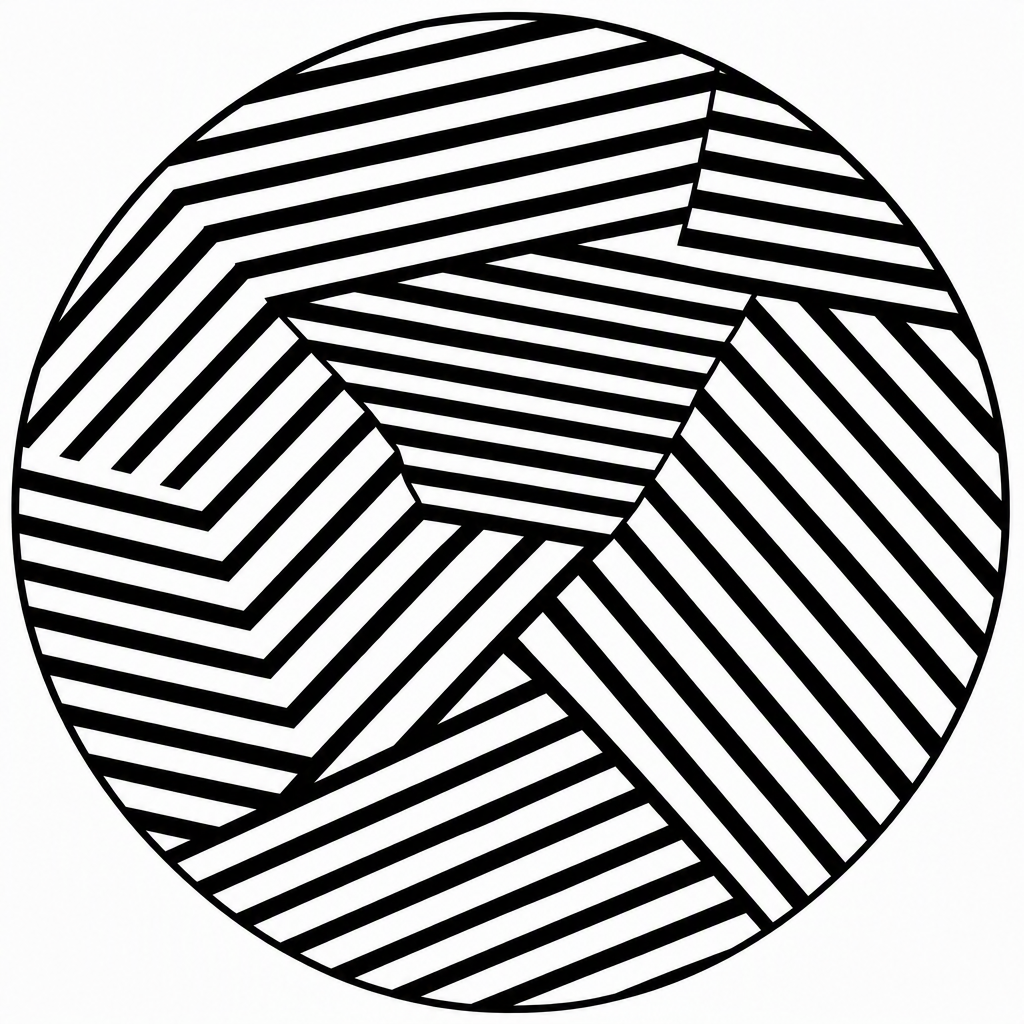
\includegraphics[width=0.1\textwidth]{../xmPictures/image.png}
\end{center}
    \begin{solution}
        Dit vinden we terug op het eutectische punt in het diagram:

        
\bigskip
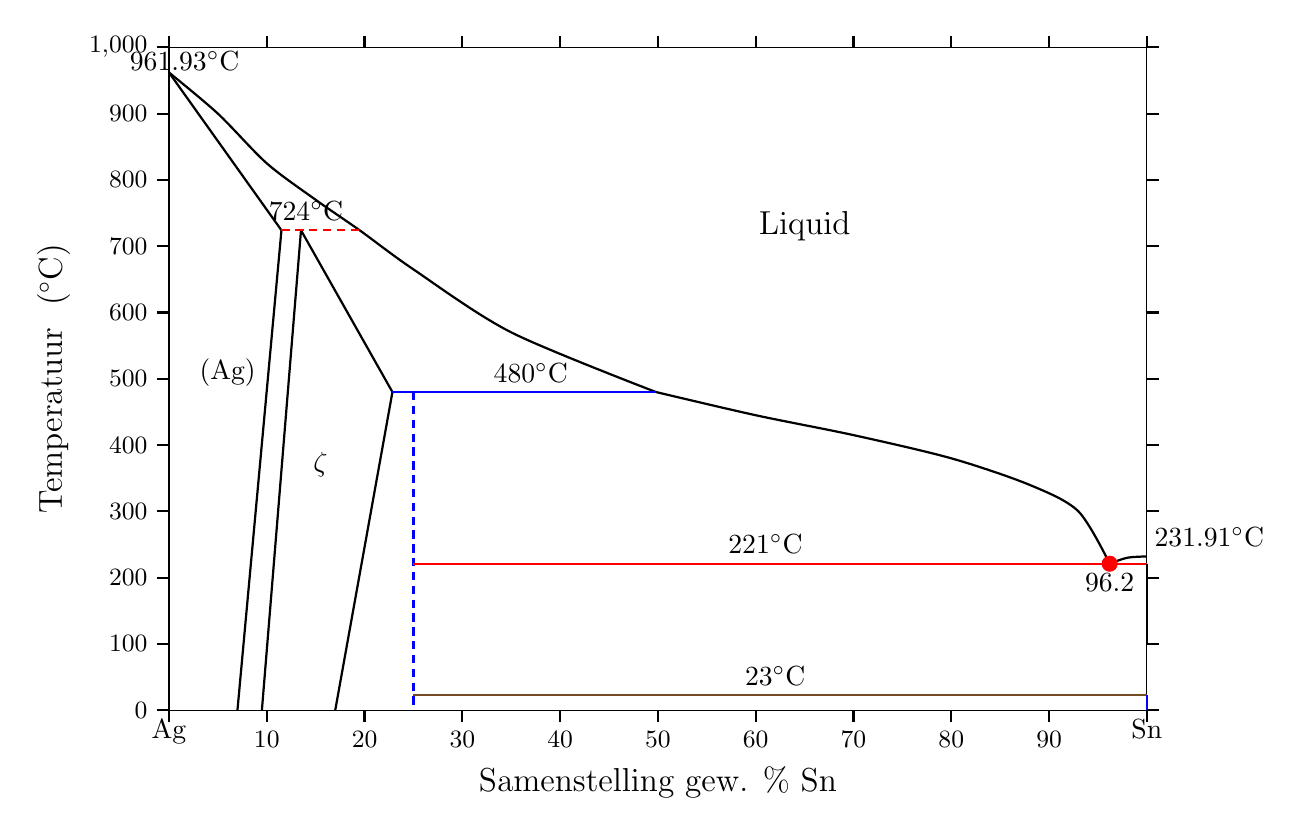
\begin{tikzpicture}
\begin{axis}[
    width=14cm, height=10cm, xmin=0, xmax=100, ymin=0, ymax=1000,
    axis lines=box,
    xlabel={Samenstelling gew. \% Sn}, ylabel={Temperatuur $\ (^\circ\mathrm{C})$},
    xtick={0,10,20,30,40,50,60,70,80,90,100},
    xticklabels={,10,20,30,40,50,60,70,80,90,},
    ytick={0,100,200,300,400,500,600,700,800,900,1000},
    minor tick num=0, tick style={black,thick}, tick align=outside,
    enlargelimits=false, clip=false,
    xlabel style={font=\large}, ylabel style={font=\large},
    tick label style={font=\small},
    every axis plot/.append style={thick, black, no marks},
]

% Liquidus curve
\addplot[smooth] coordinates {(0,962) (5,900) (10,825) (15,770) (19.5,724) (25,665) (35,570) (49.8,480)};
\addplot[smooth] coordinates {(49.8,480) (60,445) (70,415) (80,380) (88,340) (93,300) (96.2,221)};
\addplot[smooth] coordinates {(96.2,221) (98,230) (100,232)};

% Ag-rich phase boundaries
\addplot[smooth] coordinates {(0,962) (11.5,724)};
\addplot[smooth] coordinates {(11.5,724) (7,0)};
\addplot[smooth] coordinates {(13.5,724) (9.5,0)};
\addplot[smooth] coordinates {(13.5,724) (22.85,480)};
\addplot[smooth] coordinates {(22.85,480) (17,0)};
\addplot coordinates {(25,480) (25,0)};

% Horizontal phase boundaries
\addplot coordinates {(11.5,724) (19.5,724)};
\addplot coordinates {(22.85,480) (49.8,480)};
\addplot coordinates {(25,221) (100,221)};
\addplot coordinates {(25,23) (100,23)};

% Sn-rich phase boundaries
\addplot coordinates {(100,221) (100,100)};
\addplot coordinates {(100,23) (100,0)};

% Phase labels
\node at (axis cs:65,730) {\large Liquid};
\node at (axis cs:6,510) {(Ag)};
\node at (axis cs:15.5,370) {$\zeta$};
\node[below] at (axis cs:96.2,221) {96.2};

% Temperature labels
\node[above right] at (axis cs:-5,950) {961.93$^\circ$C};
\node[above] at (axis cs:14,724) {724$^\circ$C};
\node[above] at (axis cs:37,480) {480$^\circ$C};
\node[above] at (axis cs:61,221) {221$^\circ$C};
\node[above left] at (axis cs:113,232) {231.91$^\circ$C};
\node[above] at (axis cs:62,23) {23$^\circ$C};

% Element labels
\node[below] at (axis cs:0,0) {Ag};
\node[below] at (axis cs:100,0) {Sn};

% Eutectic point
\addplot[only marks, mark=*, mark size=2.5pt, red] coordinates {(96.2,221)};

\end{axis}
\end{tikzpicture}
\bigskip
    \end{solution}
\end{question}







\end{exercise}

\end{document}